
\documentclass[utf8]{frontiersSCNS} % for Science, Engineering and Humanities and Social Sciences articles
\usepackage{url,hyperref,lineno,microtype,subcaption}
\usepackage[onehalfspacing]{setspace}
\usepackage{natbib}
%\linenumbers

\def\keyFont{\fontsize{8}{11}\helveticabold }
\def\firstAuthorLast{Arroyave {et~al.}} %use et al only if is more than 1 author
\def\Authors{Raymundo Arroyave\,$^{1,*}$, Anjana Talapatra\,$^{1}$, Shahin Boluki\,$^{2}$, Pejman Honarmandi\,$^{1}$, Alexandros Solomou\,$^{3}$,  Seyede Fatemeh Ghoreishi\,$^{4}$, Douglas Allaire\,$^{4}$  Xiaoning Qian\,$^{2}$ , Edward Dougherty\,$^{2}$ , and Dimitris C. Lagoudas\,$^{1,3}$}

\def\Address{$^{1}$ Department of Materials Science \& Engineering, Texas A\&M University, 3003 TAMU,  College Station, Texas -77843 \\
$^{2}$ Department of Electrical \& Computer Engineering, Texas A\&M University, College Station, Texas -77843 \\
 $^{3}$ Department of Aerospace Engineering, Texas A\&M University, College Station, TX 77843  \\
 $^{4}$ Department of Mechanical Engineering, Texas A\&M University, College Station, Texas -77843}
% The Corresponding Author should be marked with an asterisk
% Provide the exact contact address (this time including street name and city zip code) and email of the corresponding author
\def\corrAuthor{Corresponding Author}

\def\corrEmail{raaroyave@tamu.edu}


\begin{document}
\onecolumn
\firstpage{1}

\title[Experiment Design Frameworks]{Experiment Design Frameworks for Accelerated Discovery of Targeted Materials Across Scales} 

\author[\firstAuthorLast ]{\Authors} %This field will be automatically populated
\address{} %This field will be automatically populated
\correspondance{} %This field will be automatically populated

\extraAuth{}% If there are more than 1 corresponding author, comment this line and uncomment the next one.
%\extraAuth{corresponding Author2 \\ Laboratory X2, Institute X2, Department X2, Organization X2, Street X2, City X2 , State XX2 (only USA, Canada and Australia), Zip Code2, X2 Country X2, email2@uni2.edu}


\maketitle


\begin{abstract}
Over the last decade, there has been a paradigm shift away from labor-intensive and time consuming materials discovery methods and materials exploration through informatics approaches is gaining traction at present. Current approaches  are however typically centered around the idea of achieving this exploration through high-throughput experimentation/computation. Such approaches, however, do not account for the practicalities of resource constraints which eventually result in bottlenecks at various stage of the workflow. Regardless of how many bottlenecks are eliminated, the fact that ultimately a human must make decisions about what to do with the acquired information implies that HT frameworks face hard limits that will be extremely difficult to overcome. Recently,this problem has been addressed by framing materials discovery as an optimal experiment design problem. In this article, we discuss the need for optimal experiment design, the challenges in it's implementation and finally discuss some successful examples of materials discovery via experiment design.  


\tiny
 \keyFont{ \section{Keywords:} Materials discovery, efficient experiment design, Bayesian optimization, information fusion, Materials Informatics, Machine learning} 
\end{abstract}

\section{Introduction}

 Historically, the beginning of materials research centered around learning to use the elements and minerals discovered in nature. The chief challenge at the time was the separation of  the pure metal from the mined ore which lead over time to the science of metallurgy - the foundation of current day materials research. Then, humans discovered that these pure metals could be combined to form alloys, followed by the principles of heat treatments - advances that shaped history; since the ability to invent new and exploit known techniques to use metals and alloys to forge weapons for sustenance and  defense  was instrumental in the success, expansion  and migration of early civilizations. Additionally, there is evidence that the oft quoted sequence of copper-tin bronze-iron which lend their names to the `\textit{ages}' of human progress, occurred in different parts of the world, sometimes even simultaneously \cite{tylecote1992history}. Thus, the desire to harvest materials from nature and use them to improve the quality of life is a uniquely human as well as universal trait. 

 With the acceleration of scientific advances over the last few centuries, man has moved on from developing applications based on available materials, to demanding materials to suit desired applications. Science and technology are continuously part of this contentious chicken and egg situation where it is folly to prioritize either  - scientific knowledge for its own sake or the use of science as a tool to fuel new applications. Regardless, the majority of the scientific breakthroughs from the materials perspective have resulted from an Edisonian approach and guided primarily by experience, intuition and to some extent, serendipity. Further, bringing the possibilities suggested by such discoveries to fruition takes decades and considerable financial resources. Also, such approaches when successful, enable the investigation of a very small fraction of a given materials design space leaving vast possibilities unexplored. No alchemic recipes exist, however desirable, which given a target application  and desired properties, enables one to design the optimized material for that application. However, to tread some distance on that alchemic road, recently, extensive work has centered on the accelerated and cost-effective discovery, manufacturing, and deployment of novel and better materials as promoted by the Materials Genome Initiative \cite{holdren2011materials}. 
 
 \subsection{Challenges in Accelerated Materials Discovery Techniques}

 The chief hurdle when it comes to searching for new materials with requisite or better properties is the scarcity of physical knowledge  about the class of materials that constitute the design space. Data regarding the structure and resultant properties may be available, but what is lacking is usually the fundamental physics that delineate the processing-structure-property-performance (PSPP) relationships in these materials. Additionally, the interplay of structural, chemical and microstructural degrees of freedom introduces enormous complexity, which exponentially increases the dimensionality of the problem at hand, limiting the application of traditional design strategies. 

 To bypass this challenge, the focus is on the use of data‐to‐knowledge approaches, the idea being to implicitly extract the material physics embedded in the data itself with the use of modern day tools - machine learning, design optimization, manufacturing scale-up and automation, multiscale modeling, and uncertainty quantification with verification and validation. Typical techniques include the utilization of High-Throughput (HT) computational \cite{HPE1,HPC2,HPC3} and experimental frameworks \cite{HPE1,HPE2,HPE3,HPE4}, which are used to generate large databases of materials feature / response sets, which then must be analyzed \cite{HPC4} to identify the materials with the desired characteristics \cite{solomou2018multi}. HT methods, however, fail to account for  constraints in experimental / computational) resources available, nor do they anticipate the the existence of bottle necks in the scientific workflow that unfortuantely render impossible the parallel execution of specific experimental / computational tasks. 

 Recently, the concept of optimal experimental design, within the overall framework of Bayesian Optimization (BO), has been  put forward as a design strategy to circumvent the limitations of traditional (costly) exploration of the design space. This was pioneered by Balachandran et al. \cite{balachandran2016adaptive} who put forward a framework that balanced the need to exploit available knowledge of the design space with the need to explore it by using a metric ( Expected Improvement (EI)) that selects the best next experiment with the end-goal of accelerating the iterative design process. BO-based approaches rely on the construction of a response surface of the design space and are typically limited to the use of a single model to carry out the queries. This is an important limitation, as often times, at the beginning of a materials discovery problem, there is not sufficient information to elucidate the feature set (i.e., model) that is most related to the specific performance metric to optimize. 

 Additionally, although these techniques have been successfully demonstrated in a few materials science problems \cite{MP1,MP2,MP3,MP4,MP5,MP6,MP7,MP8,MP9}, the published work tends to focus on the optimization of a single objective \cite{balachandran2016adaptive}, which is far from the complicated multi-dimensional real world materials design requirements.

In this manuscript, we discuss the materials discovery challenge from the perspective of experiment design - i.e. goal-oriented materials discovery, wherein we efficiently exploit available computational tools, in combination with experiments, to accelerate the development of new materials and materials systems. In the following sections, we discuss the need for exploring the field of Materials discovery via the experiment design paradigm and then  specifically discuss two approaches that address the prevalent limitations discussed above: i) a framework that is capable of adaptively selecting competing models connecting materials features to performance metrics through Bayesian Model Averaging (BMA), followed by optimal experimental design, ii) a framework for the fusion of information that exploits correlations among sources/models and between the sources and ‘ground truth’ in conjunction with a a multi-information source optimization framework that identifies, given current knowledge, the next best information source to query and where in the input space to query it via a novel value-gradient policy and examples of applications of these approaches in the context of single-objective and multi-objective materials design optimization problems  and information fusion in CALPHAD-based thermodynamic modeling. 

\section{Experiment Design}
 The divergence of modern science from it's roots in natural philosophy was heralded by the emphasis on experimentation in the sixteenth and seventeenth centuries as a means to establish causal relationships \cite{hacking1983representing}. Experiments involve the manipulation of one or more independent variables followed by the systematic observation of the effects of the manipulation on one or more dependent variables. An experiment design then, is the formulation of a detailed experimental plan in advance of doing the experiment that which when carried out will describe or explain the variation of information under conditions that are hypothesized to reflect the variation. An optimal experiment design maximizes either the amount of "information" that can be obtained for a given amount of experimental effort or the accuracy with which the results are obtained, depending on the purpose of the experiment. A schematic of the experiment design process is shown in Figure \ref{fig:01}.

 Taking into consideration the large number of measurements often needed in materials research, design problems are formulated as a multi-dimensional optimization problem, which typically require training data in order to be solved.  Prior knowledge regarding parameters and features affecting the desired properties of materials is of great importance. However, ofen prior knowledge is inadequate and the presence of large uncertainties is detrimental to the experimental design. Hence, additional measurements or experiments are necessary in order to improve the predictability of the model with respect to the design objective. Naturally, it is then essential to direct experimental efforts such that the targeted material may be found by minimizing the number of experiments. This may be achieved via an experimental design strategy that is able to distinguish between different experiments based upon the information they can provide. Thus, the experiment design strategy results in the choosing of the next best experiment, which is determined by optimizing an \textit{acquisition} function.

\subsection{Experiment Design under Model Uncertainty}
In most materials design tasks, there are always multiple information sources at the disposal of the material scientist. 
For example, the relationships between the crystal structure and properties/performance can in principle be developed through experiments as well as (computational) models at different levels of fidelity and resolution ( atomistic scale, molecular scale, continuum scale). Traditional holistic design approaches such as Integrated Computational Materials Engineering (ICME), on the other hand, often proceed on the limited and unrealistic assumption that there is only one source available to query the design space.
For single information sources and sequential querying, there are two traditional techniques for choosing what to query next in this context \cite{lynch2007introduction}. In most materials design tasks, there are always multiple information sources at the disposal of the material scientist. For example, the relationships between the crystal structure and properties/performance can in principle be developed through experiments as well as (computational) models at different levels of fidelity and resolution ( atomistic scale, molecular scale, continuum scale). Traditional holistic design approaches such as Integrated Computational Materials Engineering (ICME), on the other hand, often proceed on the limited and unrealistic assumption that there is only one source available to explore the design space.

In the realm of  single information sources and sequential querying, two approaches are most commonly used to choose the next query/experiment \cite{scott2011correlated}. These are  (i) efficient global optimization (EGO) \cite{jones1998efficient} and its extensions, such as sequential Kriging optimization (SKO) \cite{huang2006sequential} and value-based global optimization (VGO)\cite{moore2014value}, and (ii) the knowledge gradient (KG) \cite{frazier2008knowledge,gupta1994bayesian,gupta1996bayesian}. EGO uses a Gaussian process \cite{rasmussen2004gaussian} representation of available data, but does not account for noise \cite{schonlau1996global,schonlau1998global}. SKO also uses Gaussian processes, but includes a variable weighting factor to favour decisions with higher uncertainty \cite{scott2011correlated}. KG differs in that while it can also account for noise, it selects the next experiment on the basis of the expected value of the best material after the experiment. In the case of multiple uncertain sources of information (e.g., different models for the same problem), it is imperative to integrate all the sources to produce more reliable results \cite{dasey2007information}. In practice, there are several approaches for fusing information from multiple models. Bayesian Model Averaging (BMA) and fusion under known correlation \cite{Correlation1,Correlation2,Correlation3,Correlation4} are two such  model fusion techniques that enable robust design. These two approaches shall be discussed in detail in the following sections. 


\subsubsection{Bayesian Model Averaging (BMA)}

The goal of any materials discovery strategy  is to identify an action that results in a desired property, which is usually optimizing an objective function of the action over the Materials Design Space (MDS).  In materials discovery, each action is equivalent to an input or design parameter setup. If complete knowledge of the objective function exists, then the materials discovery challenge is met. In reality however, this objective function is a blackbox, of which little if anything is known and the cost of querying such a function (through expensive experiments/simulations) at arbitrary query points in the MDS is very high. In these cases a parametric or nonparametric surrogate model can be used to approximate the true objective function. Bayesian Optimization (BO) \cite{shahriari2016taking}  corresponds to these cases, where the prior model is sequentially updated after each experiment. 
Irrespective of whether prior knowledge about the form of the objective function exists and/or many observations of the objective values at different parts of the input space are available, there is an inherent feature selection step, where different potential feature sets might exist. Moreover, there might be a set of possible parametric families as candidates for the surrogate model. Even when employing nonparametric surrogate models, several choices for the functional form might be available. These translate into different possible surrogate models for the objective function. The common approach is to select a feature set and a single family of models and fix this selection throughout the experiment design loop; however, this is not a reliable approach due to the small initial sample size that is ubiquitous in materials science. 

This problem was addressed by framing experiment design as Bayesian Optimization under Model Uncertainty (BOMU), and incorporating Bayesian Model Averaging (BMA) within Bayesian Optimization.  The \textit{acquistion} function used is the Expected Improvement (EI) which seeks to balance the need to exploit available knowledge of the design space with the need to explore it. Suppose that $f^\prime$ is the minimal value of the objective function $f$ observed so far. Expected improvement evaluates $f$ at the point that, in expectation, improves upon $f^\prime$ the most. This corresponds to the following utility function:
\begin{equation}
I = 0, max(f^\prime - f(x))
 \end{equation}
If $\hat{y}$ and $s$ are the predicted value and it's standard error at $x$ respectively, then the expected improvement is given by:
\begin{equation}
E[I(x)] = (f^\prime - \hat{y}) \Phi \frac{(f^\prime - \hat{y})}{s} + s \phi \frac{(f^\prime - \hat{y})}{s}
\end{equation}
where: $\phi$(.) and $\Phi$(.) are the standard normal density and distribution functions \cite{jones1998efficient}. 

The  Bayesian Optimization under Model Uncertainty approach may then be described in words as follows:

\begin{itemize}
\item There is a collection of potential models (e.g. models based on different features sets)
\item The models are averaged, based on the (posterior) model probabilities based on initial data set to form a BMA.
\item Using the expected acquisition function under the BMA, an experiment is chosen that maximizes the expected acquisition.
\item The experiment is run, each model is updated and the (posterior) model probabilities are updated.
\item The expected acquisition under the updated BMA is computed and an experiment is chosen.
\item This iteration is done until some stopping criteria (e.g. while objective not satisfied and budget not exhausted), and the best observation so far is selected as the final suggestion.
\end{itemize}
Incorporating BMA within Bayesian Optimization produces a system capable of autonomously and adaptively learning not only the most promising regions in the materials space but also the models that most efficiently guide such exploration. The framework is also capable of defining optimal experimental sequences in cases where multiple objectives must be met—we note that recent works have begun to address the issue of multi-objective Bayesian Optimization [38] in the context of materials discovery. Our approach, however, is different in that the multi-objective optimization is carried out simultaneously with feature selection.
The overall framework for autonomous materials discovery is shown in Figure \ref{fig:02}. 

\subsubsection{Error correlation-based model fusion (CMF) approach}
As mentioned earlier, model-based ICME-style frameworks tend to focus on integrating tools at multiple scales under the assumption that there is a single model/tool rwhich is significant at a specific scale of the problem. This ignores the use of multiple models that may be more/less effective in different regions of the performance space. Data-centric approaches, on the other hand, tend to focus (with some exceptions) on the brute-force exploration of the MDS, not taking into account the considerable cost associated with such exploration.
In \cite{ghoreishi2018multi}, the authors presented a framework that addresses the two outstanding issues listed above in the context of the optimal microstructural design of advanced high strength steels. Specifically, they carried out the fusion of multiple information sources that connect microstructural descriptors to mechanical performance metrics. This fusion is done in a way that accounts for and exploits the correlations between each individual information source—reduced order model constructed under different simplifying assumptions regarding the partitioning of (total) strain, stress or deformation work among the phases constituting the microstructure—and between each information source and the ground truth—represented in this case by a full-field microstructure-based finite element model. This finite element model is computational, and is considered as a higher fidelity model as part of a multifidelity framework, the intention being to create a framework for predicting ground truth. Specifically, the purpose of the work was not to  match the highest fidelity model, but to predict material properties when created at ground truth. There is usually no common resource tradeoff in this scenario, in contrast to traditional computational multifidelity frameworks that trade computational expense and accuracy. 

In the framework, the impact a new query to an information source has on the fused model is of value. The search is performed over the nput domain and the information source options concurrently to determine which next query will lead to the most improvement in the objective function. In addition, the exploitation of correlations between the discrepancies of the inormation sources in the fusion process is novel and enables the identification of ground truth optimal points that are not shared by any individual information sources in the analysis.

A fundamental hypothesis of this approach is that any model can provide potentially useful information to a given task. This technique thus takes into account all potential information any given model may provide and fuses unique information from the available models. The fusion goal then is to identify dependencies, via estimated correlations, among the model discrepancies. With these estimated correlations, the models are fused following standard practice for the fusion of normally distributed data.
To estimate the correlations between the model deviations when they are unknown, the reification process \cite{allaire2012fusing,thomison2017model} is used, which refers to the process of treating each model, in turn, as ground truth. The underlying assumption here is that the data generated by the reified model represents the true quantity of interest. These data are used to estimate the correlation between the errors of the different models and the process is then repeated for each model. The detailed process of estimating the correlation between the errors of two models can be found in Refs. \cite{allaire2012fusing,thomison2017model}. A flowchart of the approach is shown in figure \ref{fig:04}. The next step then is to determine which information source should be queried and where to query it, concurrently, so as to produce the most value  with the tacit resource constraint in mind. For this decision, a utility, which is referred to as the value-gradient utility is used, which accounts for  both the immediate improvement in one step and expected improvement in two steps. The goal here is to produce rapid improvement, with the knowledge that every resource expenditure could be the last, but at the same time, to  be optimally positioned for the next resource expenditure. In this sense, there is equal weight accorded to next step value with next step (knowledge) gradient information, hence the term value-gradient. As mentioned in the previous section, in the BMA approach, the Expected Improvement (EI) metric is used to choose the next query point, while in this approach, the value gradient is used.

The knowledge gradient, which is a measure of expected improvement, is defined as:
\begin{equation}
\nu^{KG}(x) = E [V^{N+1} H^{N+1}(x)) - V^N H^N| H^N]
\end{equation}

The KG policy for sequentially choosing the next query is then given as:
\begin{equation}
x^{KG} = \arg\!\max_{x \in \chi} \nu^{KG}(x)
\end{equation}

and the value-gradient utility is given by:
\begin{equation}
U = \mu^*_{fused} + \max_{x \in \chi} \nu^{KG}(x)
\end{equation}
where $\mu^*_{fused}$ is the maximum value of the mean function of the current fused model and $\max_{x \in \chi} \nu^{KG}(x)$ is the maximum expected improvement that can be obtained with another query as measured by the knowledge gradient over the fused model. 

\subsection{ Application of Experiment Design Framework: Examples}

\subsubsection{ Multi-Objective Bayesian Optimization}

A Multi-objective Optimal Experimental Design (OED) framework (see Figure \ref{fig:05}) based on the Bayesian optimization techniques was reported by the authors in \cite{solomou2018multi}. The specific objective of this Bayesian Optimal Experimental Design (BOED) framework in this study was to provide an Optimal Experiment Selection (OES) policy to guide an efficient search of precipitation strengthened NiTi Shape memory alloys (SMAs) with selected target properties by efficiently solving a multi-objective optimization problem. The EHVI \cite{emmerich2011hypervolume} acquisition function was used to perform multi-objective optimization. EHVI balances the trade-off between exploration and exploitation for multi-objective BOED problems, similar to EI for single-objective problems. EHVI is a scalar quantity that allows a rational agent to select, sequentially, the next best experiment to carry out, given current knowledge, regardless of the number of objectives, or dimensionality, of the materials. The optimal solutions in an optimization problem are typically referred as Pareto optimal solutions or Pareto front or Pareto front points. The Pareto optimal solutions in a selected multi-objective space, correspond to the points of the objective space that are not dominated by any other points in the same space.

For the NiTi SMA, the considered input variables were the  initial homogeneous Ni concentration of the material before precipitation $(c)$ and the volume fraction $(v_f)$ of the precipitates while the objective functions were functions of the material properties of the corresponding homogenized SMA. The framework was used to  discover precipitated SMAs with (objective 1) an austenitic finish temperature $A_f = 30^\circ C$ , (objective 2) a specific thermal hysteresis that is defined as the difference of austenitic finish temperature and martensitic start temperature, $A_f - M_s = 40^\circ C$. The problem was solved for two case studies, where the selected continuous MDS is discretized with a coarse and a dense mesh respectively. The refined MDS has $n_T = 21021$ combinations of the considered variables $c$ and $v_f$ . The utility of the queried materials by the BOED framework within a predefined experimental budget is compared with the utility of the corresponding queried materials following a Pure Random Experiment Selection (PRES) policy and a Pure Exploitation Experiment Selection (PEES) policy within a predefined experimental budget. An experimental budget of is assumed of $n_B = 20$ material queries and for the case of the OES and PEES policies the experimental budget is allocated to $n_I =1$ randomly queried material and to $n_E = 19$. 

The results are indicated in Figure \ref{fig:06a}. It is seen that the OES policy, even under the limited experimental budget, queries materials that belong to the region of the objective space which approaches the true Pareto front. This is clear by comparing the Pareto front calculated based on the results of the OES (blue dash line) with the true Pareto front found during the case study 1 (red dot line). The results also show that the materials queried by the PRES policy are randomly dispersed in the objective space as  expected while the materials queried by the PEES policy are clustered in a specific region of the objective space which consists of materials with similar volume fraction values which is anticipated courtesy the true exploitative nature of the policy. On further analysis is is seen that the OES on average queries materials with better utility in comparison to the other two policies, while the PRES policy exhibits the worst performance. 

Same trends of performance are maintained through the equivalent comparisons conducted for various experimental budgets as shown  in Figure \ref{fig:06b} which also indicates similar curves for the coarse mesh. It is apparent that if the OES policy is employed to query a material in a discrete MDS with defined variables bounds, its relative performance in comparison to the PRES policy becomes more definitive as the discretization of the MDS is further refined, as the gap between PRES and OES policies for the case of the dense discretized MDS (red lines) is much bigger than that in the case of the coarse discretized MDS (blue lines) optimally queried materials. The results of the BOED framework thus demonstrate that the method could efficiently approach the true Pareto front of the objective space of the approached materials discovery problems successfully. Such treatment was also carried out for a three objective problem with the additional objective of maximizing the maximum 
saturation strain ( $H_{sat}$) that the material can exhibit and similar conclusions were drawn.


\subsubsection{ Bayesian Model Averaging: Search for MAX phase with maximum bulk modulus}
The BMA framework was demonstrated by efficiently exploring the MAX ternary carbide/nitride space through Density Functional Theory (DFT) calculations by the authors in \cite{talapatra2018autonomous}.  The problem was formulated with the goal of identifying the material/materials with the maximum bulk modulus $K$ with a resource constraint of permitting experiments totally querying 20\% of the MDS. The case of the maximum bulk modulus $K$ is designed as a single-objective optimization problem while the second problem is designed as a multi-objective problem. Features describing the relation between the material and objective functions were obtained from literature and domain knowledge. Feature correlations were used to finalize six different feature sets which are denoted as F$_1$, F$_2$, F$_3$, F$_4$, F$_5$ and F$_6$. Complete details may be found in \cite{talapatra2018autonomous}. Some representative results are shown here.  Calculations were carried out for different number of initial data instances $N  = 2,  5,  10,  15,  2$0. The performance trends for all problems across different values of N  are consistent. The technique is found to not significantly depend on quantity of initial data. Here, representative results for $N = 5$ are shown. 

Figure \ref{fig:03a} indicates the maximum bulk modulus found in the experiment design iterations based on each model (feature set) averaged over all initial data set instances for $N= 5$. The dotted line in the figure indicates the maximum bulk modulus = 300 GPa that can be found in the MDS. F$_2$ is found to be the best performing feature set on average, converging fastest to the maximum bulk modulus. F$_6$ and F$_5$ on the other hand, are uniformly the worst performing feature sets on average, converging the slowest. It is evident that using a regular optimization approach will work so long there is, apriori, a good feature set.   Unfortunately, due to small sample size and large number of potential predictive models, the feature selection step may not result in the true best predictive model for efficient Bayesian Optimization. Small sample sizes pose a great challenge in model selection due to inherent risk of imprecision and, and no feature selection method performs well in all scenarios when sample sizes are small. Thus, by selecting a single model as the predictive model based on small observed sample data, one ignores the model uncertainty. 

To circumvent this problem the Bayesian Model Averaging (BMA) method was used. Regression models based on aforementioned six feature subsets, were adopted in the BMA experiment design.  The BMA coefficients were evaluated in two ways: first-order (BMA$_1$ ) and second-order (BMA$_2$ ) Laplace approximation. Figure \ref{fig:03c}  shows the comparison of the average performance of both the first-order and second-order BMA over all initial data set instances with the best performing model ($F_2$) and worst performing model (F$_6$). It can be seen that both the first-order and second-order BMA performance in identifying the maximum bulk modulus is consistently close to the best model (F$_2$). BMA$_1$ performs as well as if not better than F$_2$. Figure \ref{fig:03d} shows the corresponding swarm plots indicating the number of calculations required to discover the maximum bulk modulus in the MDS for for $N = 5$using BMA$_1$ and BMA$_2$. It can be seen that for a very high percentage of cases the maximum bulk modulus can be found within the designated budget. In Figures \ref{fig:03e} and \ref{fig:03f}, the average model coefficients (posterior model probabilities) of the models based on different feature sets over all instances of initial data set are shown with the increasing number of calculations for BMA$_1$ and BMA$_2$ respectively.  Thus we see that, while prior knowledge about the fundamental features linking the material to the desired material property is certainly essential to build the Materials Design Space (MDS), the BMA approach may be used to auto-select the best features/feature sets in the MDS, thereby eliminating the requirement of knowing the best feature set a priori . Also, this framework is not significantly dependent on the size of the initial data, which enables its use in materials discovery problems where initial data is scant.

\subsubsection{ Multi-Source Information Fusion: Application to Dual-Phase materials}

\subsubsection{Bayesian Model Averaging and Information Fusion: CALPHAD-based thermodynamic modeling}
Calculation of phase diagrams (CALPHAD) is one of the fundamental tools in alloy design and an important component of ICME. Uncertainty quantification of phase diagrams is the first step required to provide confidence for decision making in property- or performance-based design. In work that was the first of it's kind \cite{honarmandi2019bayesian}, the authors independently generated four CALPHAD models describing Gibbs free energies for the $Hf-Si$ system. The MCMC Metropolis Hastings toolbox in Matlab was then utilized for probabilistic calibration of the parameters in the applied CALPHAD models. These results are shown for each model in Figure \ref{fig:07}where it is seen that there is a very good agreement between the results obtained from model 2 and the data with a very small uncertainty band and consequently a small Model Structure Uncertainty (MSU) \cite{choi2008inductive}. Models 3 and 4 on the other hand show large uncertainties for the phase diagrams which are mostly attributed to MPU. In the context of BMA, the weight of the applied models was
calculated to be 0.1352, 0.5938, 0.1331, and 0.1379, respectively, indicating that Model 2 thus has three times the weight of the other models, which otherwise have similar Bayesian importance, which is consistent with the phase diagram results in Figure \ref{fig:07}. The phase diagram obtained using BMA is shown in \ref{fig:08}. The posterior modes of the probability distributions in the BMA model exactly correspond to the posterior modes of the probability distributions in model 2. Thus, the best model results can be considered as the optimum results for the average model, but with broader uncertainties, contributed by the inferior models. In BMA, each model has some probability of being true and the fused estimate is a weighted average of the models. This method is extremely useful in the case of model-building process based on a weighted average over the models' responses, and/or less risk (more confidence) in design based on broader uncertainty bands provided by a weighted average over the uncertainties of the models’ responses.
Error Corrrelation-based Model fusion was then used to fuse the models together in two ways: i) Fuse models 1, 3 , 4 to examine whether the resulting fused model maybe closer to the data and reduce the uncertainties and ii) Fuse models 1,2,3 and 4 together. Figure \ref{fig:09}a  shows that the approach can provide a phase diagram in much better agreement with data and less uncertainties compared to phase diagrams obtained from each one of the applied models individually. This result implies that random CALPHAD models can be fused together to find a reasonable estimation for phase diagram instead of trial-and-error to find the best predicting model. It is also apparent that better predictions can be achieved as shown in \ref{fig:09}b if model 2 (the best model) is also involved in the model fusion. The information fusion technique allowed the acquisition of more precise estimations and lower uncertainties compared to results obtained from each individual model. 
In summary, the average model obtained from BMA shows larger 95\% con- fidence intervals compared to any one of the individual models, which can provide more confidence for robust design but is likely too conservative. On the other hand, the error correlation-based technique can provide closer results to data with less uncertainties than the individual models used for the fusion. The uncertainty reductions through this fusion approach are also veri- fied through the comparison of the average entropies (as a measure of uncertainty) obtained for the individual and fused models. Therefore, random CALPHAD models can be fused together to find reasonable predictions for phase diagrams with no need to go through the cumbersome task of identifying the best CALPHAD models.

\section{Conclusions and Recommendations}
In this work, we have reviewed some of the most important challenges and opportunities related to the concept of optimal experiment  as an integral component for the development of Materials Discovery frameworks. As our understanding of the vagaries implicit in differnt design problems progresses, tailoring experiment design strategies around the specific material classes under study while further developing the experiment design frameworks will become increasingly feasible and successful. As techniques improve, we will be able to access and explore increasingly complex materials design spaces, opening the door to precision tailoring of materials to desired applications. Challenges in the form of the availability and generation of sufficient and relevant data of high quality need to be continuously addressed. The optimal way to accomplish this would be the implementation of universal standards, centralized databases and the development of an open access data-sharing system in conjunction with academia, industry, government research institutions and journal publishing agencies which is already underway.  

\section{Conflict of Interest Statement}

The authors declare that the research was conducted in the absence of any commercial or financial relationships that could be construed as a potential conflict of interest.

\section{Author Contributions}
All authors have contributed equally to this work.
\section{Funding}

The authors acknowledge the support of NSF through the projects NSF-CMMI-1534534, NSF-CMMI-1663130, and DGE- 1545403. RA and ED also acknowledge the support of NSF through Grant No. NSF-DGE-1545403. XQ acknowledges the support of NSF through the project CAREER: Knowledge-driven Analytics, Model Uncer- tainty, and Experiment Design, NSF-CCF-1553281 and NSF-CISE-1835690 (with RA). AT and RA also acknowledge support by the Air Force Office of Scientific Research under AFOSR-FA9550-78816-1- 0180 (Program Manager: Dr. Ali Sayir). RA and DA also acknowledge the support of ARL through [grant No. W911NF-132-0018]. 

\section{Acknowledgments}
Calculations were carried out in the Texas A\&M Supercomputing Facility.

\bibliographystyle{frontiersinSCNS_ENG_HUMS} 
\bibliography{experiment_design}


\section{Figures}

\begin{figure}[!]
\centering
\includegraphics[scale=0.3]{./figures/experiment_design}
\caption{A schematic of the recursive experiment design process}
\label{fig:01}
\end{figure}

\begin{figure}[!]
\centering
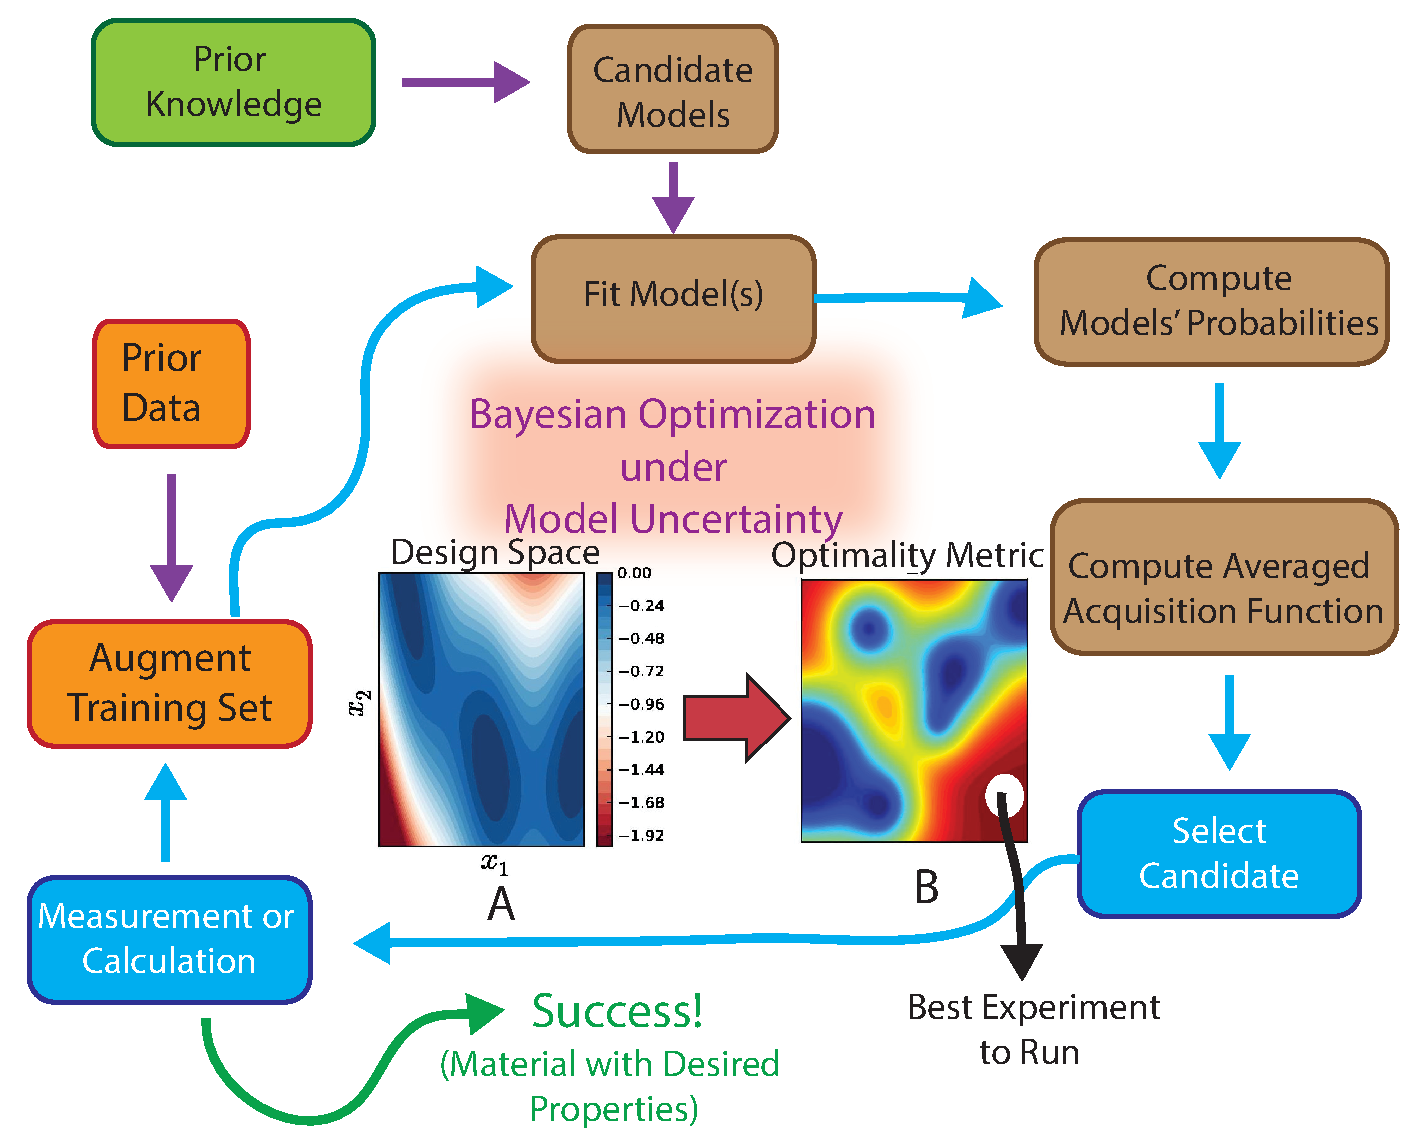
\includegraphics[scale=0.5]{./figures/BOMU}
\caption{Schematic of the proposed framework for an autonomous, efficient materials discovery system as a realization of Bayesian Optimization under Model Uncertainty (BOMU). Initial data and a set of candidate models are used to construct a stochastic representation of an experiment/simulation. Each model is evaluated in a Bayesian sense and its probability is determined. Using the model probabilities, an effective acquisition function is computed, which is then used to select the next point in the materials design space that needs to be queried. The process is continued iteratively until target is reached or budget is exhausted. Used with permission from \cite{talapatra2018autonomous}.}
\label{fig:02}
\end{figure}




\begin{figure}[!]
\centering
\includegraphics[scale=0.5]{./figures/information_fusion_flowchart}
\caption{Flowchart of the information fusion approach. Adapted from \cite{ghoreishi2018multi}}
\label{fig:04}
\end{figure}

\begin{figure}[!]
\centering
\includegraphics[scale=0.4]{./figures/Multi_objective_BO}
\caption{Autonomous closed-loop, multi-objective Bayesian Optimal Experimental Design framework. Adapted from \cite{solomou2018multi}}
\label{fig:05}
\end{figure}


\begin{subfigure}[!]
\includegraphics[scale=1]{./figures/multi_ojective_pareto.jpg}
\caption{Calculated objective space and Pareto front using the OES,
PRES and PEES policies under the $n_B = 20$ experimental budget. Reproduced with permission from \cite{solomou2018multi}}
\label{fig:06a}
\end{subfigure}%
\begin{subfigure}[!]
\includegraphics[scale=1]{./figures/multi_ojective_pareto_policies.jpg}
\caption{Comparison of the utility of the queried materials by the OES, PRES and PEES policies as function of the experimental budget for the 2-objectives materials discovery problem. Reproduced with permission from \cite{solomou2018multi} }
\label{fig:06b}
\end{subfigure}

\begin{subfigure}[!]
\includegraphics[scale=1]{./figures/N_5_K_max_single_models}
\caption{Representative results for single objective optimization -- maximization of bulk modulus for N=5: a) Average maximum bulk modulus discovered using all described feature sets,}
\label{fig:03a}
\end{subfigure}%
\begin{subfigure}[!]
\includegraphics[scale=1]{./figures/K_max_N_5}
\caption{Representative results for single objective optimization -- maximization of bulk modulus for N=5: swarm plots indicating the distribution of the number of calculations required for convergence using all described feature sets }
\label{fig:03b}
\end{subfigure}
\begin{subfigure}[!]
\includegraphics[scale=1]{./figures/N_5_K_max_BMA}
\caption{Representative results for single objective optimization -- maximization of bulk modulus for N=5: average maximum bulk modulus discovered using the best feature set $F_2$, worst feature set $F_6$, BMA$_1$ and BMA$_2$ }
\label{fig:03c}
\end{subfigure}
\begin{subfigure}[!]
\includegraphics[scale=1]{./figures/K_max_N_5_BMA_violinplot}
\caption{Representative results for single objective optimization -- maximization of bulk modulus for N=5: swarm plots indicating the distribution of the number of calculations required for convergence using the best feature set $F_2$, worst feature set $F_6$, BMA$_1$ and BMA$_2$  }
\label{fig:03d}
\end{subfigure}
\begin{subfigure}[!]
\includegraphics[scale=1]{./figures/N_5_mo_BMA_first_order_coeff}
\caption{Representative results for single objective optimization --maximization of bulk modulus for N=5: Average model probabilities for maximizing bulk modulus using BMA$_1$ }
\label{fig:03e}
\end{subfigure}
\begin{subfigure}[!]
\includegraphics[scale=1]{./figures/N_5_mo_BMA_second_order_coeff}
\caption{Representative results for single objective optimization --maximization of bulk modulus for N=5: Average model probabilities for maximizing bulk modulus using BMA$_2$ }
\label{fig:03f}
\end{subfigure}



\begin{figure}[!]
\includegraphics[scale=1]{./figures/PD_4_MCMC}
\caption{Optimum HfeSi phase diagrams and their 95\% BCIs obtained from models 1-4 (a-d) after uncertainty propagation of the MCMC calibrated parameters in each case. Reproduced with permission from \cite{honarmandi2019bayesian}}
\label{fig:07}
\end{figure}

\begin{figure}[!]
\includegraphics[scale=1]{./figures/PD_BMA}
\caption{Posterior modes and 95\% BCIs at different compositions/regions in Hf-Si phase diagram obtained after BMA.
 Reproduced with permission from \cite{honarmandi2019bayesian}}
\label{fig:08}
\end{figure}

\begin{figure}[!]
\includegraphics[scale=1]{./figures/PD_CMF}
\caption{Error correlation-based model fusions of a) three models (1, 3, and 4) and b) all four models.Reproduced with permission from \cite{honarmandi2019bayesian}}
\label{fig:09}
\end{figure}

\end{document}
